\documentclass[a5paper,12pt]{article}
\usepackage{notes}
\begin{document}
\begin{titlepage}
\begin{center}
\HRule \\[0.5cm]
\textsc{\huge Cubic Curve}\\[0.5cm]
\HRule \\[0.5cm]
\textsc{\Large Notes on the derivation of a cubic curve}\\[0.5cm]
\vfill
Hannah Michelle Ellis\\[1.0cm]
\today
\end{center}
\end{titlepage}

\clearpage
\tableofcontents
\listoftables
\listoffigures
\clearpage

\section{Geometry}
\begin{figure}[h]
  \centering
  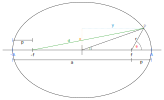
\includegraphics[width=\textwidth]{./img/diagram}
\caption{Ellipse with important points marked} \label{fig:geometry}
\end{figure}

Looking at figure \ref{fig:geometry}, we can see that
\begin{equation}
a+p=2A
\end{equation}
and
\begin{equation}
a-p=2f
\end{equation}

We can use a definition of eccentricity as the ratio of distance to the focus point over the semi major axis.

\begin{equation}
e=\frac{f}{A}
\end{equation}

One parametrisation for an ellipse is
\begin{align}
	x&=A\cos E \\ \nonumber
	y&=B\sin E
\end{align}














An ellipse can be formed by keeping the sum of the lengths of two lines from two equally spaced focal points constant. This text however will not assume that is the case and will derive the equations for an ellipse in both Cartesian and polar forms from this setup. Figure \ref{fig:Setup} shows the geometry we will start with to derive the equations.
Starting from this we note a couple of things. Firstly the sum of the lengths of each line is defined to be constant ($D$). Also the lengths of the projections onto the x axis must sum to $2f$.
\begin{framed}
\begin{equation}\label{eq:D}
d_1+d_2=D
\end{equation}
\begin{equation}\label{eq:f}
l_1+l_2=2f
\end{equation}
\end{framed}

From the geometry in figure \ref{fig:Setup}
\begin{equation}\label{eq:d1}
d_1=\sqrt{{l_1}^2+y^2}=\sqrt{(f+x)^2+y^2}
\end{equation}
\begin{equation}\label{eq:d2}
d_2=\sqrt{{l_2}^2+y^2}=\sqrt{(f-x)^2+y^2}
\end{equation}

\section{Carteisan form}

Starting with equation \ref{eq:D} and subtituting equations \ref{eq:d1} for $d_1$ and \ref{eq:d2} for $d_2$ gives

\begin{equation}
D=\sqrt{(f+x)^2+y^2}+\sqrt{(f-x)^2+y^2}
\end{equation}
taking one square root onto one side and squaring gives
\begin{subequations}
\begin{align}
\left(D-\sqrt{(f-x)^2+y^2}\right)^2=(f+x)^2+y^2\\
D^2-2D\sqrt{(f-x)^2+y^2}+(f-x)^2+\Ccancel[red]{y^2}=(f+x)^2+\Ccancel[red]{y^2}\\
D^2-2D\sqrt{(f-x)^2+y^2}+\Ccancel[blue]{f^2}-2fx+\Ccancel[green]{x^2}=\Ccancel[blue]{f^2}+2fx+\Ccancel[green]{x^2}\\
D^2-4fx=2D\sqrt{(f-x)^2+y^2}\\
\frac{D}{2}-\frac{2f}{D}x=\sqrt{(f-x)^2+y^2}
\end{align}
\end{subequations}
now we have isolated the second root, we can now square again to give
\begin{subequations}
\begin{align}
\left(\frac{D}{2}-\frac{2f}{D}x\right)^2=(f-x)^2+y^2\\
\left(\frac{D}{2}\right)^2\Ccancel[violet]{-2fx}+\left(\frac{2f}{D}\right)^2x^2=f^2\Ccancel[violet]{-2fx}+x^2+y^2\\
\left(\frac{D}{2}\right)^2+\left(\frac{2f}{D}\right)^2x^2=f^2+x^2+y^2
\end{align}
\end{subequations}
Finally group terms
\begin{subequations}
\begin{align}
\left(\frac{D}{2}\right)^2-f^2=\left(1-\left(\frac{2f}{D}\right)^2\right)x^2+y^2\\
\left(\frac{D}{2}\right)^2-f^2=\frac{\left(\frac{D}{2}\right)^2-f^2}{\left(\frac{D}{2}\right)^2}x^2+y^2\\
1=\frac{x^2}{\left(\frac{D}{2}\right)^2}+\frac{y^2}{\left(\frac{D}{2}\right)^2-f^2}\\
\end{align}
\end{subequations}
finally giving us
\begin{equation}
1=\frac{x^2}{\left(\frac{D}{2}\right)^2}+\frac{y^2}{\left(\frac{D}{2}\right)^2-f^2}\\
\end{equation}
Which is of the typical form for the Cartesian equation for an ellipse, with $A=\frac{D}{2}$ and $B=\sqrt{A^2+f^2}$. Both of which can (and will) be shown to arise from the geometry of the situation.

\subsection{The semi major axis}
\begin{figure}[h]
  \centering
\definecolor{dark_green}{rgb}{0,0.39,0}
\begin{tikzpicture}[line cap=round,line join=round,>=triangle 45,x=1.0cm,y=1.0cm,scale=2]
\draw[->,color=black] (-2.5,0) -- (3.5,0);
\draw[->,color=black] (0,-0.5) -- (0,1);s
\draw[color=blue](-2,-0.1)--(-2,0.1);
\draw[color=blue](2,-0.1)--(2,0.1);
\draw[color=blue](3,-0.1)--(3,0.1);
\draw[color=dark_green](-2,0)--(3,0);
\draw[color=dark_green](2,0)--(3,0);
\draw[->,color=orange](0,0)--(3,0);
\draw[|-|,color=black](-2,-0.8)--(3,-0.8);
\draw[|-|,color=black](2,-1.2)--(3,-1.2);
\begin{scriptsize}
\draw[color=blue](-2,-0.3) node[scale=2]{$-f$};
\draw[color=blue](2,-0.3) node[scale=2]{$f$};
\draw[color=orange](0.5,-0.2)node[scale=2]{$x$};
\draw[color=black](0.5,-0.6)node[scale=2]{$l_1$};
\draw[color=black](2.5,-1)node[scale=2]{$l_2$};
\draw[color=dark_green](0.5,0.3)node[scale=2]{$d_1$};
\draw[color=dark_green](2.5,0.3)node[scale=2]{$d_2$};
\draw[color=blue](3,-0.3)node[scale=2]{$A$};
\end{scriptsize}
\end{tikzpicture}
 
\caption{Orientating the two lines to form the semi major axis} \label{fig:semiMajor}
\end{figure}

In the situation shown in figure \ref{fig:semiMajor} we have that
\begin{subequations}
\begin{align}
d_1&=A+f\\
d_2&=A-f\\
D=d_1+d_2&=A+f+A-f=2A \label{subeq:D}
\end{align}
\end{subequations}
It imediatly follows from equation \ref{subeq:D} that $A=\frac{D}{2}$

\subsection{The semi minor axis}
\begin{figure}[h]
  \centering
\definecolor{dark_green}{rgb}{0,0.39,0}
\begin{tikzpicture}[line cap=round,line join=round,>=triangle 45,x=1.0cm,y=1.0cm,scale=2]
\draw[->,color=black] (-2.5,0) -- (2.5,0);
\draw[->,color=black] (0,-0.5) -- (0,2.5);
\draw [shift={(-2,0)},color=dark_green,fill=dark_green,fill opacity=0.1] (0,0) -- (0:1) arc (0:45:1) -- cycle;
\draw[color=blue](-2,-0.1)--(-2,0.1);
\draw[color=blue](2,-0.1)--(2,0.1);
\draw[color=dark_green](-2,0)--(0,2);
\draw[color=dark_green](2,0)--(0,2);
\draw[->,color=red](0,0)--(0,2);
\draw[|-|,color=black](-2,-0.8)--(0,-0.8);
\draw[-|,color=black](0,-0.8)--(2,-0.8);
\draw[color=blue,fill=blue,fill opacity=0.1](0.2,0)--(0.2,0.2)--(0,0.2)--(0,0)--cycle;
\draw[color=red](-0.1,2)--(0.1,2);
\begin{scriptsize}
\draw[color=dark_green] (-1.5,0.15) node[scale=2] {$\theta$};
\draw[color=blue](-2,-0.3) node[scale=2]{$-f$};
\draw[color=blue](2,-0.3) node[scale=2]{$f$};
\draw[color=red](0.2,0.8)node[scale=2]{$y$};
\draw[color=black](-1,-0.6)node[scale=2]{$l_1$};
\draw[color=black](1,-0.6)node[scale=2]{$l_2$};
\draw[color=dark_green](-1.3,1)node[scale=2]{$d_1$};
\draw[color=dark_green](1.3,1)node[scale=2]{$d_2$};
\draw[color=red](0.3,2)node[scale=2]{$B$};
\end{scriptsize}
\end{tikzpicture}
 
\caption{Orientating the two lines to form the semi major axis} \label{fig:semiMinor}
\end{figure}

In the situation shown in figure \ref{fig:semiMinor} we have that
\begin{subequations}
\begin{align}
d_2&=\frac{D}{2}=\sqrt{f^2+B^2}\\
B&=\sqrt{\left(\frac{D}{2}\right)^2-f^2}\label{eq:B}
\end{align}
\end{subequations}
as obtained above
\begin{framed}
\subsection{Summary}
In this section we have found that the equation of an ellipse in Cartesian form is
\begin{equation*}
\frac{x^2}{A^2}+\frac{y^2}{B^2}=1
\end{equation*}
Where $A$ and $B$ can be related to parameters of the constant length line formation as follows
\begin{subequations}
\begin{align*}
A&=\frac{D}{2}\\
B&=\sqrt{\left(\frac{D}{2}\right)^2-f^2}
\end{align*}
\end{subequations}
Where $D$ is the total length of the two lines connecting a point on the ellipse to the two focal points, and $f$ is the distance from origin to the two focal points.
\end{framed}
\section{Polar Form}
The polar form can be found directly from figure \ref{fig:Setup} as it is just a matter of finding the length of $d_1$ in terms of $\theta$.
Starting from equation \ref{eq:D} and substituting in \ref{eq:d2} and rearranging to get $d_1$
\begin{equation}
d_1=D-\sqrt{{l_2}^2+y^2} 
\end{equation}
using equation \ref{eq:f} to substitute for $l_2$
\begin{subequations}
\begin{align}
d_1&=D-\sqrt{(2f-l_1)^2+y^2} \\
d_1&=D-\sqrt{4f^2 - 4fl_1 + {l_1}^2+y^2}  \label{eq:polard1}
\end{align}
\end{subequations}
A quick glance at figure \ref{fig:Setup} will show that $d_1^2={l_1}^2 + y ^2$ which we can use in equation \ref{eq:polard1}.
\begin{subequations}
\begin{align}
d_1=D-\sqrt{4f^2 - 4fl_1 + d_1^2 }\\
D-d_1=\sqrt{4f^2 - 4fl_1 + d_1^2 }
\end{align}
\end{subequations}
now squaring away the square root
\begin{subequations}
\begin{align}
(D-d_1)^2=4f^2 - 4fl_1 + d_1^2 \\
D^2-2Dd_1+\Ccancel[red]{{d_1}^2}=4f^2 - 4fl_1 + \Ccancel[red]{{d_1}^2}\\
D^2-2Dd_1=4f^2 - 4fl_1\\
d_1=\frac{D^2-4f^2 +  4fl_1}{2D} \\
d_1=\frac{D}{2}-\frac{(2f)^2}{2D} +  \frac{2f}{D}l_1\\
d_1-  \frac{2f}{D}l_1=\frac{D}{2}-\frac{(2f)^2}{2D} 
\end{align}
\end{subequations}
Now we wish to get things in terms of $\theta$ by making the substitution $l_1=d_1 \cos \theta$
\begin{subequations}
\begin{align}
d_1\left(1-  \frac{2f}{D}\cos \theta \right)=\frac{D}{2}-\frac{(2f)^2}{2D} \\
d_1\left(1-  \frac{2f}{D}\cos \theta \right)=\frac{D}{2}\left(1-\frac{(2f)^2}{2D}\frac{2}{D}\right) \\
d_1\left(1-  \frac{2f}{D}\cos \theta \right)=\frac{D}{2}\left(1-\left(\frac{2f}{D}\right)^2\right)
\end{align}
\end{subequations}
finally we get the form
\begin{equation}
d_1=\frac{\frac{D}{2}\left(1-\left(\frac{2f}{D}\right)^2\right)}{1-  \frac{2f}{D}\cos \theta}\label{eq:rawPolarForm}
\end{equation}
which is exactly the polar form
\begin{equation}
r=\frac{A\left(1-e^2\right)}{1- e\cos \theta}\label{eq:polarform}
\end{equation}
with $A=\frac{D}{2}$ as before and $e=\frac{2f}{D}$

\subsection{Polar form in terms of apses}
Starting with the a slightly expanded form of equation \ref{eq:polarform}
\begin{equation} \label{eq:ellipse}
r(\theta)=\frac{A(1+e)(1-e)}{1-e \cos \theta} 
\end{equation}

When $r$ is maximums when $\cos \theta=1$ i.e. when $\theta=0$.
We stall call the maximum radius $a$ so using equation \ref{eq:ellipse} with $\cos \theta=1$
\begin{equation} \label{eq:apoasis}
a=\frac{A(1+e)(1-e)}{1-e}=A(1+e)
\end{equation}
Also we can find when $r$ is minimum. This occurs when $\cos \theta=-1$ i.e. when $\theta=\pi$. Again using equation \ref{eq:ellipse} with $\cos \theta=-1$
\begin{equation} \label{eq:periapsis}
p=\frac{A(1+e)(1-e)}{1+e}=A(1-e)
\end{equation}

We can sum the equations \ref{eq:apoasis} and \ref{eq:periapsis} above to give 
\begin{align}
a+p&=A+eA+A-eA \nonumber \\
a+p&=2A \nonumber \\
A&=\frac{a+p}{2}\label{eq:ApoPeri:semiMajorAxis}
\end{align}

This also follows from the geometry of an ellipse.

finally taking the difference of the equations \ref{eq:apoasis} and \ref{eq:periapsis} above gives
\begin{align}
a-p&=A+eA-A+eA \nonumber \\
a-p&=2eA \nonumber \\
e&=\frac{a-p}{2A} \nonumber \\
e&=\frac{a-p}{a+p} \label{eq:ApoPeri:ecentricity}
\end{align}

Using equation \ref{eq:rawPolarForm} and comparing to equation \ref{eq:polarform} gives
\begin{align}
e&=\frac{f}{A} \nonumber \\
f&=eA\nonumber \\
&=\frac{a-p}{a+p}\frac{a+p}{2} \nonumber \\
&=\frac{a-p}{2}
\end{align}

Finally we can get $B$ in terms of $a$ and $p$ by using equation \ref{eq:B}
\begin{subequations}
\begin{align}
B^2&=\left(\frac{D}{2}\right)^2-f^2 \\
B^2&=A^2-f^2 \\
B^2&=\frac{(a+p)^2}{4}-\frac{(a-p)^2}{4}\\
B^2&=\frac{a^2+2ap+p^2}{4}-\frac{a^2-2ap+p^2}{4}\\
B^2&=ap \\
B&=\sqrt{ap}
\end{align}
\end{subequations}
\begin{framed}
\subsection{Summary}

Letting $a=r_{max}$ and $p=r_{min}$ we find that these relate to other properties of the ellipse as follows
\begin{align*}
A&=\frac{a+p}{2} \\
e&=\frac{a-p}{a+p} \\
f&=\frac{a-p}{2} \\
B&=\sqrt{ap}
\end{align*}
\end{framed}
\clearpage
\addcontentsline{toc}{chapter}{Index}
\printindex
\end{document}